\chapter{Wild Approximate Inference: Why and How}
\label{chap:wild}

% **************************** Define Graphics Path **************************
\ifpdf
    \graphicspath{{Chapter5/figs/Raster/}{Chapter5/figs/PDF/}{Chapter5/figs/}}
\else
    \graphicspath{{Chapter5/figs/Vector/}{Chapter5/figs/}}
\fi

The design of approximating distributions is equally, if not more, crucial to the invention of optimisation algorithms such as the two algorithms presented in previous chapters. Mean-field approximations are often ineffective! Apparently if the $\mathcal{Q}$ family is expressive enough to contain the exact posterior, variational inference, either with KL divergence or R{\'e}nyi divergence, would return it as the only global optimum. Hence if a more complex structure is included in the q distribution, the approximation might become much more accurate and potentially even exact. For this purpose, it would be useful to use universal functional approximators, e.g.~neural networks, to expand the distribution family of approximations. However, it becomes very challenging to use these flexible approximations due to many restrictions, which cannot be addressed by simply investing more computational resources (say more running time and memory). 

In recent years, one major research direction is to go beyond mean-field methods via development of flexible $q$ distributions, which specifically addresses the intractability issues when applied to VI. For example, invertible transformations are utilised to construct $q$ distributions which allow analytical evaluations of the approximate posterior density \citep{rezende:flow2015, kingma:iaf2016, louizos:multiplicative2017}. Mixture distributions of more flexible forms are also introduced to capture the possible multi-modality of the exact posterior, with further approximations being proposed to account for extra computational challenges \citep{salimans:mcmcvi2015, tran:vgp2016, ranganath:hvm2016,maaloe:agdm2016}. Though effective, these methods are complicated for practitioners to understand, let alone the design work itself that requires lots of care.

In the second theme of the thesis, an alternative research direction will be presented towards using flexible approximations in approximate inference. Concretely, instead of designing approximate posterior distributions that fit into standard frameworks like VI, we would like to develop optimisation algorithms that enable approximations of \emph{arbitrary} form. This goal is further justified by revisiting the fundamental problem that approximate inference is trying to solve -- approximating an integral both accurately and quickly. Throughout the discussions, readers will realise that many computational constraints are irrelevant to inference itself: it is the chosen optimisation algorithm that introduces additional constraints on the $q$ distribution design. Consequently, successful development of algorithms that present no more constraints would enable the usage of \emph{arbitrary} approximate distributions, allowing practitioners to choose the $q$ distribution that fits best to their particular tasks. 
%
In the following, we will discuss several research directions towards this goal, with one specific example detailed in the next chapter. 

The rest of the chapter is organised as follows. In Section \ref{sec:chap5_wild_concept} we revisit the tractability issues in Bayesian inference and argue that \emph{fast sampling} should be the only condition required by Monte Carlo based approximate inference algorithms. Based on this observation, we suggest using \emph{implicit} distributions as approximate posterior distributions, with some examples provided in Section \ref{sec:chap5_wild_dist} to demonstrate the flexibility of this distribution class. As implicit distributions do not exhibit tractable densities, we propose a few research directions towards fitting these approximate posteriors in Section \ref{sec:chap5_wild_solutions}. Lastly we briefly discuss a research theme -- meta-learning for approximate inference algorithms -- in Section \ref{sec:chap5_wild_applications}, which is enabled by wild approximate inference methods.

\vspace{1em}
\begin{tcolorbox}
\textbf{Remark} (Related work)\textbf{.}
The material in this chapter was originally presented in a NIPS 2016 approximate inference workshop abstract ``Wild Variational Approximations'' which is a joint work with Qiang Liu \citep{li:wild2016} (see publication page). Before that the research scheme had not been established in a formal way, except for very few attempts \citep{ranganath:ovi2016, wang:amortisedsvgd2016}. Later on, several groups explored an approach that blends VI and (adversarial) density ratio estimation \citep{huszar:implicit2017, tran:implicit2017, mescheder:avb2017, karaletsos:adversarial_mp2016, shi:kivi2018}, which corresponds to one of the algorithmic options described in this chapter. We argue that our work is more formal and general: we justify this line of research by examining the central topics in approximate inference, and point out four research directions for developing algorithms that can fit arbitrary $q$ distributions that enable fast sampling.
\end{tcolorbox}

\section{Revisiting tractability issues in approximate inference}
\label{sec:chap5_wild_concept}

In Chapter \ref{chap:intro} the definition of an approximate inference procedure is identified. However, here I invite the readers to consider the following question again:
\begin{center}
\emph{What does tractability mean for an approximate inference algorithm?}
\end{center}

This question touches the fundamental principles of approximate inference and it is very important answer it carefully. It helps us to understand the challenges that we face, and identify those that can be addressed by investing more \emph{computational} resources, and those that require advanced \emph{mathematical} tools. 
%
Think about the history of neural networks research as an analogy. The first challenge in the late 1960s came from \emph{theoretical} limitations of perceptrons \citep{minsky:perceptrons1969}, and the second issue in the last ten years of the 20th century was mainly the lack of \emph{computational resources} (e.g.~slow computers and small datasets) \citep{lecun:deeplearning2015}. It was only after identifying and addressing these two issues (back-propagation \citep{rumelhart:backprop1986}, faster machine, GPU computing and big data) that the deep learning community started to revolutionise AI applications in the real world. But still, there are mathematical and computational challenges for modern deep learning which are waiting for discoveries and solutions, but these issues are out of the scope of our discussions.

To answer the above question, we first start by revisiting the definition of \emph{approximate inference}, with Bayesian posterior inference as an illustrating example. Assume a model with prior distribution $p(\z)$ and likelihood function $p(\x | \z)$. Then \emph{inference} means computing the expectation of some function $F(\z)$ of interest under the exact posterior, which is $\mathbb{E}_{p(\z|\x)} [ F(\z)]$. 
Examples of such $F$ functions include $F(\z) = \z$, $F(\z) = \z \z^{\text{T}}$ (i.e.~computing the moments of $p$), $F(\z) = p(\y^*|\z, \x^*)$ if in supervised learning and $\z$ represents the model parameters (i.e.~computing a predictive distribution), and $F(\z) = \delta_{A}$ if one wishes to evaluate the distribution directly $p(\z \in A | \x) = \mathbb{E}_{p(\z | \x)}[ \delta_{A} ]$.
%
For simplicity in the rest of the discussion we assume the evaluation of $F(\z)$ can be done using available computational resources, otherwise it needs more approximations.

%
The core idea of (optimisation based) approximate inference is to fit an approximate posterior distribution $q(\bm{z}|\bm{x})$ in a ``tractable'' distribution family $\mathcal{Q}$ to the exact posterior $p(\z | \x)$, such that $\mathbb{E}_{p(\z|\x)}[F(\z)]$ can be well approximated by
\begin{equation}
\mathbb{E}_{p(\z|\x)}[F(\z)] \approx \mathbb{E}_{q(\z|\x)}[F(\z)]. 
\label{eq:chap5_approx_predict}
\end{equation}
Critically, the primary tractability requirement here for the approximate posterior is the \emph{fast computation} of the \emph{approximate expectation} on the RHS given the function $F$.

Historically, approximate distributions of simple forms, such as mean-field approximations and factorised Gaussians \citep{jordan:vi1999}, have been proposed to obtain analytical solutions of the approximated expectation. These approaches often require the probabilistic model to comprise conjugate exponential families, which excludes a broad range of powerful models, e.g.~those which warp noise variables through non-linear mappings. Instead, modern approximate inference introduces Monte Carlo (MC) estimation techniques to approximate the predictive likelihood \citep{paisley:bbvi2012,ranganath:bbvi2014} that we reviewed in Section \ref{sec:chap2_mcvi}. The MC method enables a wider class of models to be amendable to VI (the requirement is that the log-joint can be computed point-wise), and is key to modern training methods of generative models such as deep latent variable models. \citep{kingma:vae2014, rezende:vae2014}.
%

Precisely, at inference time, the MC approximation method samples $\{\z^1, ..., \z^K \}$ from the approximate posterior $q$, and estimates the required quantity by
\begin{equation}
\mathbb{E}_{q(\z|\x)}[F(\z)] \approx \frac{1}{K} \sum_{k=1}^K F(\z^k), \quad \z^k \sim q(\z|\x).
\label{eq:chap5_approx_predict_mc}
\end{equation}
Consequently, this converts the fast expectation computation requirement to \emph{fast sampling} from the approximate posterior, as the expectation is further approximated by the empirical average. Fast sampling is arguably a stronger condition compared to \emph{fast expectation computation} for a \emph{given} function $F$. 
%
The latter option typically prefers traditional numerical integration methods since for different functions one would select different quadrature rules. On the other hand, fast sampling can also be a weaker condition: once we have obtained the samples from the approximate posterior, we can use them to compute an empirical estimate of the expectation for \emph{any} integrable function. Hence methods that entail fast sampling might be preferred for tasks that require estimating expectations of a set of functions.

Unfortunately, except a few very recent attempts that will be detailed later, most approximate inference algorithms impose further constraints to the design of $q$. For example, MC-VI requires \emph{fast density evaluation} and/or \emph{fast density gradient evaluation} for $q(\z | \x)$ given a configuration of $\z$. Importantly, this requirement is only presented in the VI optimisation procedure to seek for the best fit of $q$: once a (local) optimum is obtained, inference only requires evaluating the empirical expectation, thus there is no need to compute the density point-wise. Therefore the MC inference at test time enables the usage of \emph{implicit distributions} \citep{diggle:prescribe_implicit1984,mohamed:gan2016} and \emph{stochastic regularisation techniques (SRTs)} \citep[e.g.~dropout techniques, see][]{srivastava:dropout2014, wan:dropconnect2013, singh:swapout2016, krueger:zoneout2017, kingma:variational_dropout2015, gal:uncertainty2016} that allow for the computation of the MC predictive inference but not for fast density evaluation. But again at training time they are not applicable to traditional variational methods due to the fast density evaluation constraint. 

These observations raise an outstanding research question: 
\begin{center}
\emph{Can we design efficient approximate inference algorithms to train arbitrary posterior approximations (including implicit distributions and SRTs)?}
\end{center}

We will answer this in the next sections, by discussing proposals for training \emph{wild approximate inference algorithms}.\footnote{Not to be confused with \emph{black-box} variational inference \citep{ranganath:bbvi2014}.} We will also provide some examples of implicit posterior approximations that are not possible to be fitted using conventional approximate inference algorithms. Before that, I first address potential skepticism below, and argue why this is an outstanding but under-examined research direction.

\vspace{1em}
\begin{tcolorbox}
\textbf{Remark} (a comparison between implicit distributions and SRTs)\textbf{.}
As presented, it is desirable to remove the fast density evaluation constraint from the fitting procedure. However the reasons for doing so are different for implicit distributions and SRTs. First for implicit distributions, MC samples $\z^1, ..., \z^K$ are generated (e.g.~by warping noise variables with a neural network), in order to compute the empirical estimate $\frac{1}{K} \sum_{k=1}^K F(\z^k)$. The fast density evaluation constraint becomes an obstacle for fitting implicit distributions, as the underlying distribution of the samples does not exhibit a tractable form. 

On the other hand, in Bayesian neural networks the function $F$ is usually defined using the outputs of the neural network, i.e.~$F(\z) = \frac{1}{N} \sum_{n=1}^N \tilde{F}(\y_n = \text{NN}_{\z}(\x_n))$. Unlike implicit distributions, SRTs often apply random transformations to the hidden units, which leads to random outputs $\y_n^k, n=1, ..., N, k=1, ..., K$ and the empirical estimate $\frac{1}{KN} \sum_{k=1}^K \sum_{n=1}^N \tilde{F}(\y_n^k)$. More importantly, the random transformations applied to \emph{different} inputs $\x_n$ are \emph{different}, which is equivalent to sampling $NK$ sets of weights $\z^{k, n}, n=1, ..., N, k=1, ..., K$ \emph{implicitly}. 
%
Therefore even the underlying density of $\z^{k, n}$ might be tractable point-wise (consider Gaussian dropout \citep{srivastava:dropout2014, kingma:variational_dropout2015} as an example), evaluating them explicitly would cost $\mathcal{O}(NK)$ time or $\mathcal{O}(NK)$ memory for parallel computing. Therefore the fast density evaluation constraint becomes an obstacle again but for a different reason: intractability due to limited computational budget.
\end{tcolorbox}

\subsection{Is it necessary to evaluate the approximate posterior distribution?}

One might argue that having an accessible $q$ distribution allows the user to understand the properties of the exact posterior better. It might be true for low dimensional cases, as we can easily visualise the density function, and compare density values between samples to determine which is more probable. But I would disagree with this argument for the scenario of approximating multi-modal posterior distributions in high dimensions, which is often the application regime of interest. Some reasons are:
\begin{itemize}
\item First, enforcing the tractable density constraint means that in many cases, either we fit the posterior with a rather simple distribution (which has limited representational power), or a complex model such as a mixture density (which entails high computational costs). 

\item Second, even when setting aside the computational issues for density evaluation, visualising high dimensional distributions is itself still an open research problem. In this regard, many data visualisation techniques consider dimension reduction methods such as principal component analysis (PCA) \citep{pearson:pca1901}, self-organising map \citep{kohonen:som1998, venna:som2003} and t-SNE \citep{maaten:tsne2008}, which in fact only require samples from the distribution, not the density values. 

\item Finally as motivated above, many MC-based inference tasks do not require evaluating or comparing density values on samples. For those which do require density evaluation, one can then fit a density estimator on the samples from $q$. It can still be very convenient as in the MC estimation setting we typically assume fast sampling from the approximate posterior.
\end{itemize}

\subsection{Comparisons to sampling-based methods}
Many Bayesian statisticians prefer sampling methods -- and in fact it is the emergence of sampling methods such as importance sampling (IS), sequential Monte Carlo (SMC) \citep{doucet:smc2001} and Markov chain Monte Carlo (MCMC) that contributed to the rapid development of Bayesian statistics. They have very nice theoretical guarantees, for example, IS and SMC provide unbiased estimates of the integral and are asymptotically exact when the number of samples $K \rightarrow +\infty$. MCMC has similar asymptotic exactness guarantee but it also requires the number of transitions $T \rightarrow +\infty$. However, I view all these sampling methods as approximate inference algorithms, simply due to the fact that in practice one can never obtain an infinite number of samples, nor can one simulate the MCMC dynamics for an infinite amount of time. Furthermore, even some of these methods do construct \emph{implicit} approximate posterior distributions in practice, they still add more constraints to the inference procedures, detailed in below.

\begin{itemize}
\item (Adaptive) importance sampling (IS) and sequential Monte Carlo (SMC). \\
Importance sampling has a long history in statistics, e.g.~see \cite{geweke:mc1989}. Roughly speaking, it proposes samples from a rather simple distribution $\pi(\z | \x)$, then ``corrects'' the sampling estimate by incorporating the importance weight
\begin{equation}
\mathbb{E}_{p(\z|\x)}[F(\z)] \approx \frac{1}{K} \sum_{k=1}^K w_k F(\z^k), \quad w_k = \frac{p(\z^k | \x)}{\pi(\z^k | \x)}, \quad \z^k \sim \pi(\z | \x).
\label{eq:chap5_is_estimator}
\end{equation}
One can easily see the unbiasedness of the IS estimate, and under mild conditions one can also show it is consistent. Also self-normalised IS is sometimes used to obtain approximate posterior samples, which effectively constructs $q$ as 
\begin{equation}
q(\z | \x) = \sum_{k=1}^K \hat{w}_k \delta(\z = \z^k), \quad \hat{w}_k = \frac{w_k}{\sum_{k=1}^K w_j}, \quad \z^k \sim \pi(\z | \x).
\end{equation}
In this case the $q$ distribution depends on the proposal $\pi$ and the number of samples $K$, and again under mild conditions $q \rightarrow p$ when $K \rightarrow +\infty$. In this case the estimation is no longer unbiased, but practically the self-normalised IS estimate often enjoys the advantage of lower variance. Importantly, the $q$ distribution is tractable and requires fast evaluation of the $\pi$ density (up to a potentially unknown normalising constant). SMC can be viewed as importance sampling applied to time-series models (such as hidden Markov models), typically with extra techniques to improve sample efficiency.

However, IS and SMC provide terrible approximations to the desired integral if the proposal $\pi$ is very different from the target distribution $p$, mainly due to the high variance of the estimator. To address this issue, researchers have considered adapting the initial distribution to reduce the variance, therefore improving sample efficiency that is key to the success of IS in practice, Indeed the (unnormalised) optimal proposal distribution for IS is proportional to $| F(\z) | p(\z | \x)$, and in some cases the resulting estimator has zero variance, indicating that it requires only one (!) sample to compute the exact integral. Recently there is a plenty of research work on how to adapt the initial distribution and combine the approach with amortised inference \citep{cornebise:smc2009, gu:nasmc2015, burda:iwae2016, paige:smc2016, le:aesmc2017, naesseth:vsmc2017, maddison:fivo2017}. But still, the tractability constraint of $\pi(\z | \x)$ largely restricts its analytic form to those have been used for VI.

\item Markov Chain Monte Carlo (MCMC). \\
An MCMC algorithm for posterior sampling is typically specified by a \emph{transition distribution} (or transition kernel) $\mathcal{T}(\z' | \z)$, with the following conditions often assumed:
\begin{itemize}
\item[(i)] $\mathcal{T}$ has the target distribution $p(\z|\x)$ as the \emph{unique} stationary distribution:
$$ p(\z' | \x) = \int \mathcal{T}(\z' | \z) p(\z | \x) d \z. $$
\item[(ii)] If defining 
$$ \mathcal{T}_{T}(\z_T | \z_0) = \int \prod_{t=0}^{T-1} \mathcal{T}(\z_{t+1} | \z_t) d \z_{0:T-1},$$
then for any initial distribution $q_0(\z | \x)$ the MCMC dynamics converges to the target distribution as $T \rightarrow +\infty$:
$$\lim_{T \rightarrow +\infty} q_{T}(\z | \x) = p(\z | \x), \quad q_{T}(\z | \x) := \int \mathcal{T}_{T}(\z | \z') q_0(\z' | \x) d \z' . $$
\end{itemize}
Conditions that such transition kernel $\mathcal{T}$ requires are described in e.g. chapter 11 of \cite{gelman:bda1995} and \cite{brooks:mcmcbook2011}.

In practice one often specifies an initial distribution $q_0(\z | \x)$ to draw starting particles, and stops simulating the transitions after $T$ steps according to his/her computational budget. Consequently, this truncated Markov chain also induces an implicit $q$ distribution
\begin{equation}
q(\z | \x) = \int \mathcal{T}_{T}(\z | \z') q_0(\z' | \x) d \z' .
\end{equation}
In many applications the computational budget only allows simulations of a small number of transitions, e.g.~when training big models with EM. Thus having a rapidly mixed chain would significantly reduce $T$, and to achieve this goal a lot of work has explored different designs of the transition kernel, to name a few see \cite{ahn:sgfs2012, duane:hmc1987, neal:mcmc2011, girolami:riemann_hmc2011, ding:sgnht2014}. However, these methods are often designed as a generic sampling algorithm, which might not be best suited for e.g.~sampling from Bayesian neural network posterior distributions.
\end{itemize}

Observing the above, I would argue that recent advances of sampling-based inference method do not achieve the best \emph{speed-accuracy trade-off} that is one of the most important topics in approximate inference. Indeed there are two potential directions to improve an MCMC procedure. First, as we will not be able to obtain the exact posterior from $T$-step MCMC simulations anyway, removing the asymptotic exactness requirement can potentially allow the best fit of the transition kernel, which makes $q(\z | \x) = q_{T}(\z | \x)$ the best approximator to the exact posterior in such a $\mathcal{Q}$ class. Second, even when the transition kernel is constrained to leave the exact posterior invariant, learning the transition kernel would enable fast convergence and bias reduction for the MCMC algorithm.
%
These examples are closely related to meta-learning \citep{schmidhuber:thesis1987, bengio:meta1992, naik:meta1992, thrun:meta1998} for approximate inference, which is further discussed in Section \ref{sec:chap5_wild_applications}.
%
Similarly for IS, there exist estimators that use some ``super-efficient'' weights to enable significantly faster convergence rates than $\mathcal{O}(K^{-\frac{1}{2}})$ the usual convergence rate for the IS estimator (\ref{eq:chap5_is_estimator}) \citep{del:smc2006, liu:bbis2017, ohagan:bayesian_quadrature1991, ghahramani:bayesianMC2003, oates:mc_integration2017}. More specifically, the recipe provided by \cite{liu:bbis2017} does not require a tractable initial distribution $\pi$ at all. Although these estimators can be biased, in practice they often provide better speed-accuracy trade-off due to their better sample efficiency.

%In summary, from an approximation perspective, it is also an interesting to allow constructions of implicit initial distributions and transition kernels for sampling-based inference methods. We leave it to future investigations, and in the following we only discuss wild approximate inference methods to directly fit an approximate posterior.


\section{Examples of implicit distributions}
\label{sec:chap5_wild_dist}
In this section we provide further examples of implicit distributions that can be fitted to the exact posterior using the algorithmic proposals introduced later.
%
As a reminder, we use $\vparam$ to denote the parameters for $q$, and will explicitly write $q(\z|\x) = q_{\vparam}(\z | \x)$ when necessary. 

Ultimately for any uni-variate distribution, the sampling process can be described by deterministically transforming a uniform noise variable with the inverse \emph{cumulative density function} (CDF) or quantile function:
\begin{equation}
z \sim p(z) \quad \Leftrightarrow \quad u \sim \text{Uniform}(0, 1), \quad z = \text{CDF}_{p}^{-1}(u).
\end{equation}
For multivariate distributions, a similar process would return a set of possible configurations $\text{CDF}_{p}^{-1}(u) = \{ \inf ~ \z : \text{CDF}_{p}(\z) \geq u \}$, and one could then uniformly sample from it. However, computing the (inverse) CDF can be even harder than evaluating the density $p(\z)$ at a given configuration. Nevertheless, the observation above inspires us to define the approximate distribution $q$ by transforming a random noise variable $\bm{\epsilon}$ through a deterministic mapping $\f$:
\begin{equation}
\z \sim q(\z | \x) \quad \Leftrightarrow \quad \bm{\epsilon} \sim \pi(\bm{\epsilon}), \quad \z = \f(\bm{\epsilon}, \x).
\end{equation}
This definition exhibits similar flavour as the reparameterisation trick \citep{kingma:vae2014}, and in the following we will also say $q$ is \emph{reparameterisable} if the sampling process of $q$ follows the above procedure.

An important note here is that $\f$ might not be invertible, which differs from the invertible transform techniques discussed in \citep{rezende:flow2015,kingma:iaf2016}. Thus the $q$ density cannot be evaluated by just calculating the Jacobian matrix as in the other case. It also implies that one cannot directly apply VI to find the best mapping $\f$ simply because the entropy term $\mathbb{H}[q]$ is again intractable.%\footnote{For non-invertible $\f$, directly applying the Jacobian terms to the entropy equations (like what is done for invertible transforms) would over-estimate the entropy, thus losing the lower-bounding guarantee of VI.} 
%
Thus additional mathematical tools are required to handle this type of approximations, which will be detailed in later sections. 

\subsection{Neural network transform with noise inputs}
The simplest way to define the transformation $\f$ is to construct a deterministic deep neural network $\text{NN}_{\vparam}$ which takes both the observation $\x$ and the noise variable $\bm{\epsilon}$ as input:
\begin{equation}
\z \sim q(\z | \x) \quad \Leftrightarrow \quad \bm{\epsilon} \sim \pi(\bm{\epsilon}), \quad \z = \text{NN}_{\vparam} (\bm{\epsilon}, \x).
\end{equation}
The density network \citep{mackay:density1999} further generalises this idea using ``Bayesian'' neural networks, by putting a prior distribution on the neural network parameters. In this case the sampling procedure changes to
\begin{equation}
\z \sim q(\z | \x) \quad \Leftrightarrow \quad \bm{\epsilon} \sim \pi(\bm{\epsilon}), \bm{W} \sim \pi(\bm{W}), \quad \z = \text{NN}_{\bm{W}} (\bm{\epsilon}, \x).
\end{equation}
%
Since neural networks are well known to be universal functional approximators \citep{hornik:universal_approx1989}, the hope is that the constructed neural network is expressive enough to learn how to return a point in the set of $ \text{CDF}_{p}^{-1} \circ \text{CDF}_{\pi}$. This type of distributions is also called \emph{variational programs} in \citep{ranganath:ovi2016}, or \emph{implicit generative models} in the generative model context \citep{mohamed:gan2016}. 

\subsection{Stochastic deep neural networks and recurrent neural networks}
There has been a number of recent work that investigated latent variable models as $q$ distributions, e.g.~see \cite{salimans:mcmcvi2015, ranganath:hvm2016, tran:vgp2016, maaloe:agdm2016}. In short, the $q$ distribution is constructed by a series of conditional probabilities
\begin{equation}
q(\z | \x) = \int q(\z, \z_0, \z_1, ..., \z_{T-1} | \x) d\z_{0:T-1} = \int q(\z | \z_{T-1}, \x) \prod_{t=1}^{T-1} q(\z_{t} | \z_{t-1}, \x) d\z_{0:T-1}.
\end{equation}
In the remainder of this section we will also write $\z_T = \z$. The most general form allows $q(\z_{t} | \z_{t-1}, \x)$ to have a different form at each time step $t$. Previous uses of this type of approximate distribution focused on the simple case where $q(\z_{t} | \z_{t-1}, \x)$ has tractable density (so that for small $T$ the $q$ distribution is explicit). We review some of the algorithms for fitting them in Appendix \ref{chap:optional}.

What if $q(\z_t | \z_{t-1}, \x)$ is implicit? Following the discussions of neural network approximations to the inverse CDF function, generally one can implicitly define the conditional distribution using a neural network taking $\z_{t-1}$ and an extra ``nuisance'' noise variable $\bm{\epsilon}_t$ as the input:
\begin{equation}
\z_{t} \sim q(\z_t | \z_{t-1}, \x) \quad \Leftrightarrow \quad \z_t = \f_{t}(\z_{t-1}, \bm{\epsilon}_t, \x). \quad \bm{\epsilon}_t \sim \pi(\bm{\epsilon}_t).
\end{equation}
The joint distribution $q(\z_{0:T} | \x)$ is then parameterised by a stochastic deep neural network. Again the marginal distribution $q(\z_T | \x)$ does not have a tractable density so that traditional approximate inference methods do no apply.

An interesting special case of the stochastic neural network approach considers tying the parameters of $q(\z_t|\z_{t-1}, \x)$ at every time step, which essentially makes the network a stochastic recurrent neural network (RNN). In fact this special case can be viewed as a truncated Markov chain, making the stochastic RNN approach closely related to MCMC. Although we will never be able to achieve the exactness guarantee for an MCMC algorithm, we can still use the intuition there to design an approximate $q$ distribution that works well for our data. For example, \cite{ma:mcmc_recipe2015} claimed that a stochastic gradient MCMC (SG-MCMC) algorithm within the It\^{o} diffusion framework can be framed into the following form (with discretisation)
\begin{equation}
\z_{t} = \z_{t+1} + \zeta_t [ (\bm{D}(\z_t) + \bm{Q}(\z_t) ) \nabla_{\z_t} \log p(\z = \z_t | \x) + \Gamma(\z_t) ] + \sqrt{2 \zeta_t \bm{D}(\z_t)} \bm{\epsilon}_t, \quad \bm{\epsilon}_t \sim \mathcal{N}(\bm{0}, \mathbf{I}),
\label{eq:chap5_mcmc_recipe}
\end{equation}
where $\bm{D}(\z_t)$ and $\bm{Q}(\z_t)$ control the drift and diffusion of the dynamics, and $\Gamma(\z_t)$ is a correction term to ensure asymptotic exactness (with infinitesimal discretisation step-size).
%
But recall that asymptotic exactness is not required if one only cares about the approximation quality of $q_T(\z|\x)$.
%
This inspires us to derive the following stochastic RNN using NN-defined drift and diffusion: with $\nabla_t$ short-hands for $ \nabla_{\z_t} \log p(\z = \z_t | \x)$,
\begin{equation}
\z_{t} = \z_{t+1} + \zeta_t \f_1 (\z_t, \x, \nabla_t) +  \zeta_t \f_2 (\z_t, \x, \nabla_t) \bm{\epsilon}_t, \quad \bm{\epsilon}_t \sim \mathcal{N}(\bm{0}, \mathbf{I}),
\end{equation}
with each of the $\f_i$ functions parameterised by a neural network, or even an RNN with memory modules \citep{hochreiter:lstm1997, graves:ntm2014}. A promising direction would consider learning this stochastic RNN based approximate posterior distribution so that it generalises well to unseen target distributions. This meta-learning task can be addressed in a similar fashion as in \citet{andrychowicz:gradient2016, li:optimize2016} -- see discussions in later sections and an initial experiment in Chapter \ref{chap:grad_approx}. 

\vspace{1em}
\begin{tcolorbox}
\textbf{Remark} (stochastic gradient descent (SGD) as an approximate inference method)\textbf{.}
SG-MCMC has a close relationship to SGD in that it can be viewed as adding a properly scaled noise term to a (pre-conditioned) SGD procedure. Therefore one can also draw inspiration from SGD for approximate posterior design. Indeed recently \cite{maclaurin:sgd2016} has shown that the end points obtained by early stopping SGD (i.e.~using finite $T$) results in a nonparametric variational posterior approximation. Later \cite{mandt:sgd2016, mandt:sgd2017} also showed that under some constraints, the stationary distribution of SGD also forms an approximation to the posterior. The authors further proposed tuning the parameters (learning rate, pre-conditioning matrix, etc.) using variational inference. Similar results have also been discussed in \citet{smith:sgd2018}.
\end{tcolorbox}
%

\subsection{Learning to pass messages}

An important research direction of graphical models is the fast computation of the marginal distributions of the random variables associated with the nodes in a graph. In formula, given a graphical model with graph $G = (V, E)$, marginal inference means the computation of $p(x_i) = \int p(x_i, \x_{\backslash i}) d \x_{\backslash i}$ for all $i \in V$.
%
Message passing methods, such as belief propagation and EP as reviewed in the first theme, are popular approximate inference methods for such a purpose. Historically these graphs are constructed to have simple functions attached to each factor, making the computation of local messages tractable and fast. But the message computation is no longer analytic if non-linear mappings are adopted to describe the conditional distributions or potentials. Though not a primary focus of this chapter, below we discuss two recent approaches handling this challenging case with non-conventional methods, of which both do not require tractable densities of the messages or beliefs.

\begin{itemize}
\item Adversarial training for message approximation. \\
In directed graphical model setting, we often specify the model distribution as $p(\x) = \prod_{i} p(x_i | \text{pa}(x_i))$, in which $\text{pa}(x_i)$ represent the variables attached to the parent nodes of $x_i$ in the graph. Given observed variables $\x_{o}$, we utilise the graphical structure to design $q(\x) = q(\x_o) \prod_{i \not\in o} q(x_i | \tilde{\text{mb}}(x_i))$ where $\tilde{\text{mb}}(x_i)$ denotes the variables in the Markov blanket of $x_i$ needed for d-separation given $\x_o$, and the goal is to make $q$ as close as possible to $p$. Assuming an implicit $q$ density here, a naive idea defines a \emph{global} Jensen-Shannon divergence \citep{lin:jensen_shannon1991} then using the generative adversarial network (GAN) \citep{goodfellow:gan2014} idea to (approximately) minimise it. However computing this global divergence needs an ``interpolated'' distribution $m(\x) = \frac{1}{2} p(\x) + \frac{1}{2} q(\x)$, which effectively destroys the graphical structure and thus requires the discriminator to take the entire set of variables $\x$ as the input. This can be very computationally demanding for very big graphs. Instead, \cite{karaletsos:adversarial_mp2016} sketched an algorithm using \emph{local} Jenson-Shanon divergences between $q(x_i, \tilde{\text{mb}}(x_i))$ and $p(x_i, \text{pa}(x_i))$,\footnote{In general $q(x_i, \tilde{\text{mb}}(x_i))$ can be unnormalised (usually happens in message passing), and one can define divergences between unnormalised densities accordingly, see \citet{minka:divergence2005}. } where a GAN approximation for this divergence requires only inputs for a subset of variables $\{ x_i, \text{pa}(x_i), \tilde{\text{mb}}(x_i) \}$ thus can be nested into a message passing procedure. This idea can also be extended to EP/SEP (see Chapters \ref{chap:background} and \ref{chap:factor_tying}), in which we replace the M-projection step by minimising $\mathrm{JS}[\tilde{p}_n(\mparam) || q(\mparam)]$ that is further approximated by a GAN procedure.

\item Discriminative learning of the messages. \\
Learning the parameters of an undirected graphical model often requires (loopy) belief propagation (LBP) repeatedly to infer the unobserved variables, which can be computationally challenging. However, notice that in many supervised learning tasks the latent variables are mostly served as a feature representation for later usage, in which for a test datum LBP is executed to obtain this embedding anyway. Therefore the prediction pipeline only requires the ``approximate model'' returned by message passing, and never touches the true distribution of the graphical model. Observing this, \cite{zheng:crf_rnn2015} and \cite{dai:embed_infer2016} proposed directly training the ``approximate model'' in an end-to-end fashion using supervision data. In particular, \cite{song:kbp2011} took the intuition from kernel mean embeddings \citep{smola:kernel_embedding2007} that a distribution can be summarised with a point in a reproducing kernel Hilbert space (RKHS), and proposed a belief propagation algorithm to estimate the RKHS embeddings of marginal distributions. The graph neural network \citep{gori:graph2005, scarselli:graph2009, li:gated2015, dai:embed_infer2016} further extended this idea and parameterised the outgoing belief features as neural networks taking the incoming belief features as inputs. \\
%
We note that this idea is \emph{different} from directly using $q$ as the underlying model. Unless the graph exhibits a tree structure (where $q$ converges to $p$), the local beliefs obtained from LBP might not be \emph{consistent}, i.e.~these pseudo marginals \emph{do not} always come from the same joint distribution. Rather, the modelling pipeline still uses an intractable but valid graphical model, where the discussed algorithms focus on improving the predictive inference performance directly.

\end{itemize}


\section{Algorithmic options for fitting arbitrary posterior approximations}
\label{sec:chap5_wild_solutions}
The implicit distributions discussed in Section \ref{sec:chap5_wild_dist} cannot be fitted using many existing approximate inference methods such as MC-VI. In this section, we discuss four algorithmic options for training these approximations to the posterior.\footnote{Again we note here that the discussed options are applicable to tractable $q$ distributions as well. See discussions in the remark in Section \ref{sec:chap5_wild_concept}.}
%
One of the schemes is further developed in the next chapter. Other approaches that my colleagues and I proposed (following these ideas) include \citet{li:dropout2017, li:amcmc2017} which are not presented in the thesis due to page limit. 

\subsection{Energy approximation}
Assume $q$ is reparameterisable,\footnote{For non-reparameterisable distributions $\nabla_{\bm{\phi}} \f$ can be computed with further approximations such as the generalised reparameterisation trick \citep{ruiz:generalized_reparam2016}.} i.e. $\z \sim q_{\vparam}(\z|\x) \Leftrightarrow \z = \f_{\vparam}(\x)$.
%
Then by the chain rule, the gradient of a given objective function $\mathcal{L}(\vparam)$ w.r.t.~$\vparam$ is $\nabla_{\bm{\phi}} \mathcal{L} = \nabla_{\bm{\phi}} \f \nabla_{\f} \mathcal{L} $. Therefore, if we have an approximation $\hat{\mathcal{L}}$ to the objective function, then we can approximate the gradient as $\nabla_{\bm{\phi}} \mathcal{L} \approx \nabla_{\bm{\phi}} \f \nabla_{\f} \hat{\mathcal{L}}$. We name this approach as \emph{energy/objective approximation}.

Since the loss function $\mathcal{L}(\vparam)$ is often defined as $\mathcal{L}(q_{\vparam})$, a naive method of energy approximation considers density estimation of $q_{\vparam}$ and a direct plug-in of the approximate density to the energy function. Typically a density estimator $\hat{q}$, e.g. kernel density estimators (KDE) \citep{fukunaga:mean_shift1975} or neural density estimators \citep{mackay:density1999, larochelle:nade2011}, is fitted to the samples $\{\bm{z}^k = \f(\bm{\epsilon}^k, \bm{x}) \} \sim q$, and the gradient of $\log q$ is approximated as $\nabla_{\bm{\phi}} \log q(\bm{z}|\bm{x}) \approx \nabla_{\bm{z}} \log \hat{q}(\bm{z}|\bm{x}) \nabla_{\bm{\phi}} \f$. One might even want to directly estimate $\log q$ if it turns out to be more accurate. However, practitioners should be careful with implementations using automatic differentiation tools, since the parameters of the density estimator $\hat{q}$ should not be differentiated through (even though they might depend on the samples $\bm{z}^k$). 

The next idea considers analytical approximations to (part of) the energy function, e.g.~the entropy term $\mathbb{H}[q]$ or the KL-divergence $\mathrm{KL}[q||p_0]$ in $\mathcal{L}_{\text{VI}}$, and let the MC approach handle the rest. In MC-dropout \citep{gal:dropout2016} $\mathrm{KL}[q||p_0]$ is approximated by an $\ell_2$ regulariser of the neural network weights. In \citet{li:dropout2017} we extended this framework to $\alpha$-divergence methods with further approximations. Due to the page limit, we skip the detailed discussions of this work.


A new direction for energy approximation applies density ratio estimation methods \citep{qin:ratio1998, sugiyama:ratio2009, sugiyama:ratio2012}. This is done by introducing an auxiliary distribution $\tilde{q}$ and rewriting the variational lower-bound:
\begin{equation}
 \quad \mathcal{L}_{\text{VI}}(\bm{\theta}, q; \bm{x}) =  \mathbb{E}_{q} \left[ \log \frac{p_0(\bm{z}) p(\bm{x}|\bm{z} ; \bm{\theta})}{\tilde{q}(\bm{z}|\bm{x})} + \log \frac{\tilde{q}(\bm{z}|\bm{x})}{q(\bm{z}|\bm{x})} \right].
\end{equation}
The auxiliary distribution $\tilde{q}$ is required to have tractable density and is easy to sample from. Then one can use sample-based density ratio estimation methods to fit an estimator $\tilde{R}$ to the ratio between $\tilde{q}$ and $q$. The gradient approximation for general $\tilde{q}$ distributions can be derived similarly as
\begin{equation}
 \nabla_{\bm{\phi}} \mathcal{L}_{\text{VI}} = \mathbb{E}_{q} \left[ \nabla_{\bm{\phi}} \log \frac{p_0(\bm{z}) p(\bm{x}|\bm{z}; \bm{\theta})}{\tilde{q}(\bm{z}|\bm{x})} + \nabla_{\bm{z}} \tilde{R}(\bm{z}) \nabla_{\bm{\phi}} \f \right].
\end{equation}
%
A simple example considers $\tilde{q} = p_0$ and the classification approach for ratio estimation. In short, we train a classifier 
$$D(\bm{z} \text{ sampled from } p_0 ~|~\z, \x) = (1 + \exp[-\tilde{R}(\bm{z})])^{-1}$$
to distinguish samples from $p_0$ and $q$. A related approach is the adversarial auto-encoder \citep{makhzani:adversarial_ae2015} which uses the prior distribution as an auxiliary. However, the objective function proposed in \citet{makhzani:adversarial_ae2015} replaces the $\mathrm{KL}[q||p_0]$ in the variational lower-bound with Jensen-Shannon divergence \citep{lin:jensen_shannon1991}, which lacks a justification from a Bayesian point of view.\footnote{An optimal transport \citep{villani:optimal_transport2008} perspective of adversarial auto-encoders is presented in \citet{tolstikhin:wae2018}. } Also the density ratio estimation idea can be extended to a sequence of auxiliary distributions (in a similar spirit to annealed importance sampling \citep{neal:ais2001}), which can also be adapted slowly during training to obtain a better approximation.

\vspace{1em}
\begin{tcolorbox}
\textbf{Remark} (concurrent work on the density ratio estimation idea)\textbf{.}
Since the presentation of the original material at the NIPS 2016 approximate inference workshop, this density ratio estimation proposal has also been independently considered in \cite{karaletsos:adversarial_mp2016, mescheder:avb2017, huszar:implicit2017, tran:implicit2017}. Specifically in the adversarial variational Bayes (AVB) paper \citep{mescheder:avb2017}, the authors first considered prior distribution as the auxiliary $\tilde{q}$, then discussed an advanced technique termed as \emph{adaptive contrast}, which takes $\tilde{q}$ as a Gaussian approximation to $q$. In this case the estimation of $\tilde{q}$ requires many samples from $q$ which can significantly slow down training. To address this issue, the authors further constructed a specific type of implicit $q$ distributions, which allows sharing of randomness between different $q(\z_n | \x_n)$ distributions and thus reducing the total number of MC samples computed on a mini-batch of data. This trick improves the approximation accuracy by a significant margin as density ratio estimation is accurate when the two distributions are similar to each other.
\end{tcolorbox}

\subsection{Direct gradient approximation}
\label{sec:chap5_grad_approx}
The recent development of machine learning algorithms, including VI and SG-MCMC, relies on advanced optimisation tools such as stochastic gradient descent with adaptive learning rates. Informally the optimisation procedure works as the following: given the current mini-batch of data, we first compute the gradients, then feed them to the optimiser to construct the final update of the training parameters. In the above energy approximation example, this gradient computation is done by first approximating the original objective function $\hat{\mathcal{L}} \approx \mathcal{L}$, then differentiating this approximate energy to obtain an approximate descending direction. However, even when $\hat{\mathcal{L}}$ approximates $\mathcal{L}$ very well at the points visited by gradient descent, the approximate gradient $\nabla_{\vparam} \hat{\mathcal{L}}$ can still be a poor estimator for the exact gradient $\nabla_{\vparam} \mathcal{L}$. We depict this phenomenon in Figure \ref{fig:chap_wild_loss_pathology}. Recall that practically, an optimiser only visits \emph{finite} number of locations in the parameter space. As one would typically use a deep neural network to approximate the exact loss function, without careful control the deep net can potentially overfit to the observed evaluations, leading to strongly biased gradient updates and bad local optima.

\begin{figure}
\centering
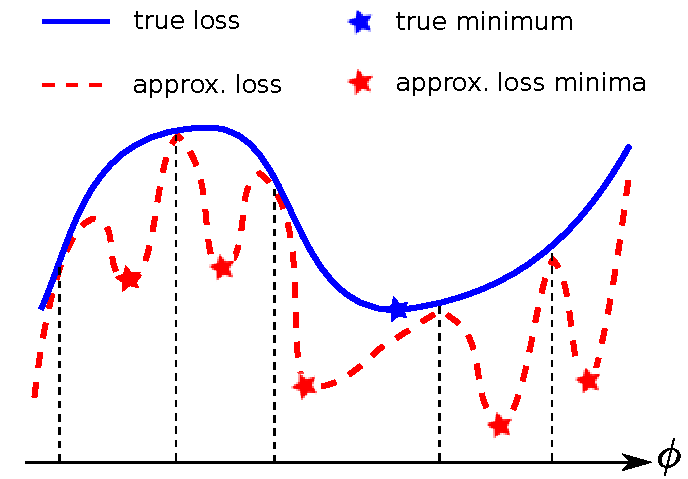
\includegraphics[width=0.5\linewidth]{Chapter5/approx_loss.pdf}
\caption{A visualisation of the exact/approximate loss. See main text for further intuition.}
\label{fig:chap_wild_loss_pathology}
\end{figure}

Here are two concrete examples for further explanation.

\begin{itemize}
\item Variational EM as an approximation to MLE. \\
The VAE algorithm can be viewed as an approximate MLE procedure, with the maximum likelihood objective $\mathcal{L}(\mparam) = \mathbb{E}_{\data}[\log p_{\mparam}(\x)]$ approximated by the variational lower-bound $\hat{\mathcal{L}}(\mparam, \vparam) = \mathbb{E}_{\data}[\mathcal{L}_{\text{VI}}(q_{\vparam}(\z | \x); \x)]$. As shown in the mean-field example in Section \ref{sec:chap4_mean_field}, this would bias the generative model $p_{\mparam}(\z | \x)$ towards simple solutions, unless $q_{\vparam}(\z | \x)$ perfectly approximates the exact posterior which is rarely the case. This issue is related to the ``hidden unit over-pruning'' problem \citep{burda:iwae2016, sonderby:ladder_vae2016}: even when $\z$ is of relatively high dimensions like a hundred, the VAE algorithm would turn off many of them, and learn a model which effectively uses much fewer units.

\item GAN training. \\
Recently generative adversarial networks (GANs) \citep{goodfellow:gan2014} have attracted large attention from the deep learning community. In a nutshell, the original GAN algorithm proposes training the generator $p_{\mparam}(\x)$ by minimising the Jensen-Shannon divergence
\begin{equation}
\min_{\mparam} \mathcal{L}(\mparam) = \mathrm{JS}[p_{\data} || p_{\mparam}] = \frac{1}{2} \mathrm{KL}\left[ p_{\data} || \frac{p_{\data} + p_{\mparam}}{2} \right] + \frac{1}{2} \mathrm{KL}\left[ p_{\mparam} || \frac{p_{\data} + p_{\mparam}}{2} \right].
\end{equation}
However, the generative model $p_{\mparam}(\x)$ is implicitly defined in an analogous way as the deterministic transform discussed above. Thus point-wise evaluation of $p_{\mparam}(\x)$ is intractable. Then the seminal GAN paper proposes approximating the Jenson-Shannon divergence \citep{lin:jensen_shannon1991} with a variational lower-bound, described by a \emph{discriminator}:
\begin{equation}
\min_{\mparam} \max_{\vparam} \hat{\mathcal{L}}(\mparam, \vparam) = \mathbb{E}_{\data} [\log D_{\vparam}(\x)] + \mathbb{E}_{p_{\mparam}} [\log (1 - D_{\vparam}(\x))].
\label{eq:chap5_original_gan}
\end{equation}
\cite{arjovsky:gan_problems2017} pointed out a fundamental problem with this approach: since both $p_{\data}$ and $p_{\mparam}$ have low-dimensional support in a high-dimensional space, the discriminator, if powerful enough (which is typically the case when using neural networks), is very likely to overfit, thus it can perfectly separate the two support sub-spaces and provide meaningless gradients. Then in their follow-up work \cite{arjovsky:wgan2017} proposed the Wasserstein GAN (WGAN), which uses Wasserstein distance \citep{villani:optimal_transport2008} as the training objective, and in this case, the approximate loss function turns out to be
\begin{equation}
\min_{\mparam} \max_{\vparam: || D_{\vparam}||_L \leq 1} \hat{\mathcal{L}}(\mparam, \vparam) = \mathbb{E}_{\data} [D_{\vparam}(\x)] - \mathbb{E}_{p_{\mparam}} [D_{\vparam}(\x)].
\label{eq:chap5_wgan}
\end{equation}
This modification, when adding more tricks to enforce the constraint $|| D_{\vparam}||_L \leq 1$ such as a gradient penalty \citep{gulrajani:wgan_gp2017}, has largely solved the instability issue of GAN training.

Another interesting explanation for why WGAN works is that the power of the discriminator, or the test function $D_{\vparam}$, has been restrained. On the other hand, in the original GAN case, over-fitting frequently happens, particularly at the beginning of training, as neural network classifiers can easily fit almost any data, even that with random labels as claimed by \cite{zhang:understanding2017}. Since smoothness is typically lost when over-fitting appears, it leads to poor approximations to the actual gradient and then a bad-performing model. Indeed \cite{kodali:dragan2017} also showed that the original GAN training can be stabilised when the discriminator is also constrained to be $1$-Lipschitz. 

\end{itemize}

From the above two examples, we see that the energy approximation approach can be problematic if not done in a correct way, therefore a \emph{direct gradient approximation} to the exact gradient might be preferred. There exists a rich literature on (non-parametric) derivative estimation \citep{stone:spline1985, zhou:spline2000, ruppert:lpr1994, fan:local_poly1996, debrabanter:lpr2013}; however, many of them require at least a noisy version of $\log q$ at the sampled locations, which is intractable in our case. Instead, \cite{singh:kernel_gradient1977} applied a kernel estimator directly to the first and higher order derivatives, and \cite{sasaki:gradient2015} improved upon this idea by performing kernel ridge regression directly on the derivatives. 
%
Also \cite{hyvarinen:score2005} considered score matching methods for approximating $\nabla_{\z} \log q(\z | \x)$, where follow-up papers \citep{sasaki:gradient2014, strathmann:kmc2015} derived kernel-based solutions and applied them to tasks such as approximate Bayesian computation (ABC) \citep{beaumont:abc2002}.
%
The core idea of these methods is the use of integration by parts to avoid evaluations of the actual gradients, making them applicable in our context. In Chapter \ref{chap:grad_approx} we will further discuss gradient approximation techniques and propose new gradient estimators for implicit models and wild approximate inference.

\vspace{1em}
\begin{tcolorbox}
\textbf{Remark} (denoising auto-encoder as a score function estimator)\textbf{.}
It has been shown in \citet{sarela:denoising2005, alain:denoising2014} that denoising auto-encoders (DAEs) \citep{vincent:denoising2008}, once trained, can be used to compute the score function approximately. Briefly speaking, a DAE learns to reconstruct a datum $\x$ from a corrupted input $\tilde{\x} = \x + \sigma \bm{\epsilon}, \bm{\epsilon} \sim \mathcal{N}(\bm{0}, \mathbf{I})$ by minimising the mean square error. Then the optimal DAE can be used to approximate the score function as $\nabla_{\x} \log p(\x) \approx \frac{1}{\sigma^2} (\text{DAE}^*(\x) - \x)$. \cite{sonderby:mapsr2016} deployed this idea to train an implicit model for image super-resolution, providing some promising results in some metrics. However applying similar ideas to variational inference can be very expensive, because the estimation of $\nabla_{\z} \log q(\z | \x)$ is a sub-routine for VI which is repeatedly required.
\end{tcolorbox}

\subsection{New optimisation objectives}
In variational inference, the KL-divergence $\mathrm{KL}[q||p]$ is minimised to obtain the approximate posterior. In general, the KL-divergence minimisation can be replaced by other optimisation-based approximation methods, as long as with the guarantee of recovering the exact posterior if $\mathcal{Q}$ contains it. However simply replacing the objective with some other $f$-divergence \citep{csiszar:divergence1963, morimoto:divergence1963, ali:divergence1966} does not simplify the problem as $q$ has an intractable density. Variational and adversarial techniques for estimating $f$-divergences \citep{nguyen:divergence2007, nguyen:divergence2010, nowozin:fgan2016} do not apply either, as the exact posterior is difficult to sample. 

One promising direction is to replace the KL divergence with Stein discrepancy \citep{stein:stein_method1972, barbour:stein_method1988, gorham:stein_method2015}, which has a special form that does not require evaluating $q$ nor sampling from $p$. 
Briefly speaking, Stein discrepancy involves a linear functional operator $\mathbf{O}_p$, called Stein operator, on a set of test functions $\mathcal{H} = \{ h(\z) \}$ such that $\mathbb{E}_{p(\bm{z}|\bm{x})}[(\mathbf{O}_p h)(\bm{z})] = 0$ for $\forall h \in \mathcal{H}$. Then the associated \emph{Stein discrepancy} is defined as $\mathcal{S}(q,  p) = \sup_{h \in \mathcal{H}} \mathbb{E}_{q}[(\mathbf{O}_p h)(\bm{z})]$. 
For continuous density functions, a generic Stein operator derived from Stein's identity \citep{stein:stein_method1972, stein:stein_method_multi1981} is $(\mathbf{O}_p h)(\z) = \nabla_{\z}\log p(\z, \x) h(\z) + \langle \nabla, h(\z) \rangle$, for which $\mathbb{E}_{p(\bm{z}|\bm{x})}[(\mathbf{O}_p h)(\bm{z})] = 0$. Putting them together, we have the Stein discrepancy (equipped with norm $|| \cdot ||$) \citep{gorham:stein_method2015}
\begin{equation}
\mathcal{S}(q, p) = \sup_{h \in \mathcal{H}} || \mathbb{E}_{q} [ \nabla_{\z}\log p(\z, \x) h(\z) + \langle \nabla, h(\z) \rangle ] ||,
\label{eq:chap5_stein_discrepancy}
\end{equation}
which only requires samples from $q$ and the score function $\nabla_{\z} \log p(\z, \x)$ and is thus indeed tractable.

Very recently Stein's method has been introduced to the approximate inference community. \cite{ranganath:ovi2016} defined $\mathcal{H}$ as parametric functions represented by neural networks, and obtained an approximate posterior by solving $\min_{q} \mathcal{S}(q, p)$. The authors approximated the minimax optimisation with gradient descent in an analogous way to GAN training \citep{goodfellow:gan2014}. In contrast, analytic solution of the supremum in (\ref{eq:chap5_stein_discrepancy}) exists if $\mathcal{H}$ is defined as the unit ball in an RKHS, where \cite{liu:ksd2016} and \cite{chwialkowski:ksd2016} termed the corresponding measure as the kernelised Stein discrepancy (KSD) that will be further discussed in Chapter \ref{chap:grad_approx}. \cite{liu:two_wild2016} further developed an approximate inference algorithm by directly minimising the KSD between the exact and approximate posterior distributions.

\subsection{Amortising stochastic dynamics}
MCMC and particle-based approximate inference methods \citep{dai:pmd2015, liu:svgd2016}, though very accurate, become inefficient when inference from multiple different distributions is repeatedly required. As an example consider learning a (deep) generative model, where fast (approximate) marginalisation of latent variables is desirable. Here we consider amortised inference to learn an inference network to mimic a selected stochastic dynamics. More precisely, we sample $\z \sim q(\z|\x)$, simulate $T$-step stochastic dynamics to obtain the updated particle $\z_{T}$, and update the $q$ distribution to ``catch-up'' those updated particles. For example, \cite{wang:amortisedsvgd2016} used this idea to amortise a deterministic dynamics called Stein variational gradient descent (SVGD) \citep{liu:svgd2016}, where the ``catch-up'' step is defined by deliberately chaining the gradients $\bm{\phi} \leftarrow \bm{\phi} + \epsilon \mathbb{E}_{q} [ \nabla_{\bm{\phi}} \bm{z} (\z_T - \z) ] $. In  \citet{li:amcmc2017} we extended this principle to MCMC methods and introduced different update rules for the (implicit) $q$ distribution. The theoretical intuition behind this approach is illustrated in Figure \ref{fig:chap5_amc_cartoon}. Since the MCMC ``oracle'' always improves the sample quality in terms of approximating the target distribution, by following the MCMC dynamics, the $q$ distribution will also get improved, until the stage when $\z_T$ has the same distribution as $\z$ which means $q = p$. Similar intuition also applies to other deterministic dynamics as long as they generate particles that are always approaching to the target distribution.

\begin{figure}
\centering
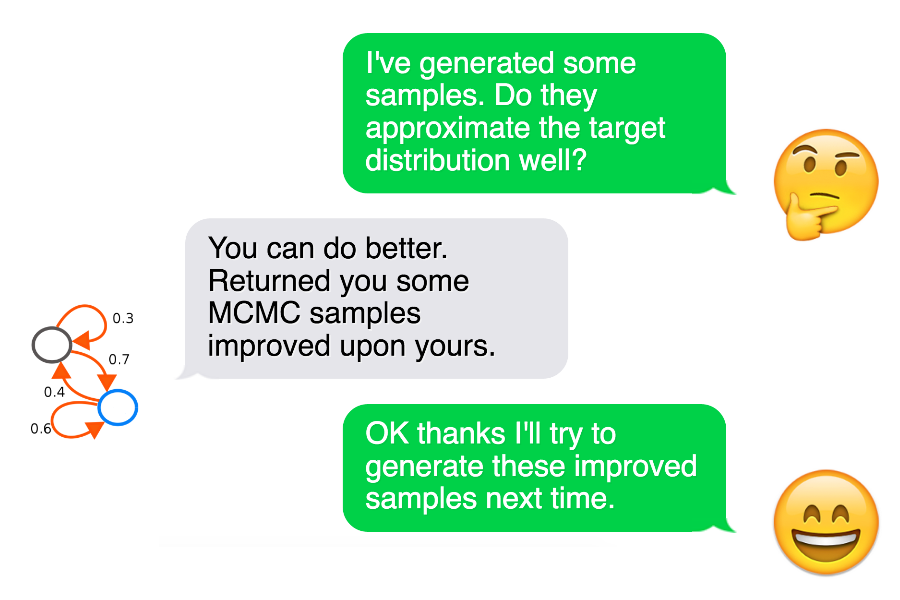
\includegraphics[width=0.6\linewidth]{Chapter5/amccartoon.png}
\caption{A cartoon illustration of the amortised MCMC idea in \cite{li:amcmc2017}. }
\label{fig:chap5_amc_cartoon}
\end{figure}



\section{Application: meta-learning for approximate inference}
\label{sec:chap5_wild_applications}

Many inference algorithms discussed in this thesis, e.g.~variational inference (with KL or R{\'e}nyi divergences) and sampling (importance sampling, SMC, MCMC, etc.), are designed as generic algorithms that can be directly applied to any integration problem. Can we automate the design of inference algorithms that are tailored to specific types of machine learning tasks (e.g.~Bayesian neural network regression)? In this section we briefly discuss a meta-learning \citep{schmidhuber:thesis1987, bengio:meta1992, naik:meta1992, thrun:meta1998} approach towards this goal.
%
The research scope of meta-learning is very broad, but in general the idea is to train a \emph{learner} on one or multiple tasks, in order to acquire common knowledge on \emph{how} to learn and generalise the learner to future tasks. Therefore meta-learning enables an inference algorithm to exploit commonly shared dependencies in a class of densities (say the posterior distribution of Bayesian neural network weights), and it is expected to produce a better approximation to the exact posterior.

In approximate inference context we define a learner as an algorithm $\mathcal{A}: \mathcal{P} \rightarrow \mathcal{Q}$ that maps the target distribution $p \in \mathcal{P}$ to an approximate distribution $q \in \mathcal{Q}$. For example, the classic variational inference algorithm can be rewritten as
\begin{equation}
\mathcal{A}_{\text{VI}}(p(\z | \x)) = \argmax_{q \in \mathcal{Q}} \mathbb{E}_q \left[ \log \frac{p(\x, \z)}{q(\z)} \right].
\end{equation}
Also the $T$-step simulation of an MCMC procedure with kernel $\mathcal{T}$ and initial distribution $q_0(\z | \x)$ is 
\begin{equation}
\mathcal{A}_{\mathcal{T}, T, q_0}(p(\z | \x)) = \int \mathcal{T}_T(\z | \z') q_0(\z' | \x) d\z' .
\end{equation}
Often these algorithms are approximated executed, e.g.~for variational inference the maximisation operator is approximated by $T$-step gradient ascent.

We consider meta-learning for approximate inference, which optimises $\mathcal{A}$ on a set of training densities $\{ p_n(\z) \}_{n=1}^N$, and generalises the learned algorithm $\mathcal{A}^*$ to unseen distributions. The training densities might come from a multi-task learning set-up, i.e.~$p_n(\z) = p(\z | \data_n)$ where $\data_n$ is the dataset for task $n$. Then one can define $\mathcal{A}(p(\z | \data)) = q_{\vparam}(\z | \data)$ with e.g.~a neural network, and then optimise the associated variational parameters $\vparam$ on the datasets $\data_1, ..., \data_N$. Further approximation techniques such as coresets \citep{huggins:coresets2016} and inducing points \citep{snelson:sparse_gp2006} can also be utilised If the dataset $\data_n$ is very big. In this case meta-learning for approximate inference algorithms can be viewed as amortised inference on \emph{task} level, therefore many of the recently developed techniques can be deployed. But it might require the use of techniques discussed in previous sections, as one might prefer the learned algorithm $\mathcal{A}$ to produce implicit posterior approximations to the target densities.

In general the $p_n$ densities might be derived from different probabilistic models with different observations and different latent variables, and the above neural network parameterisation is very likely to be sub-optimal. Instead of directly parameterising the $q$ distributions, we propose learning an approximate inference algorithm $\mathcal{A}_{\vparam}$ based on optimisation and/or sampling. 
%
%The first proposal takes inspirations from $f$-divergences \citep{csiszar:divergence1963} and the recently proposed perturbative variational objective \citep{bamler:perturbative_bbvi2017} that provides a lower-bound to the log marginal $\log p_n(\data_n)$:
%\begin{equation}
%\mathcal{A}_{f}(p_n(\z | \data_n)) = \argmax_{q \in Q} \ \mathbb{E}_q \left[ \log f \left( \frac{p_n(\data_n, \z)}{q(\z)} \right) \right]
%\end{equation}
%subject to that $f$ is a concave function on $\mathbb{R}^{+}$. A meta-learning approach would parameterise $f(\cdot) = f_{\vparam}(\cdot)$ and learn the parameters $\vparam$ by optimising some meta-objective $\mathcal{L}_{\text{meta}}$ on $\mathcal{A}_{f_{\vparam}}(p_n(\z | \data_n))$ for all $n = 1, ..., N$. Thus the learned variational objective will encourage the $q$ distribution to have desirable properties, e.g.~better interpolation between mode-seeking and mass-covering behaviours.
%
Consider learning a Markov process for posterior inference as an example. By parameterising $\mathcal{T}_n(\z'_n | \z_n) = \mathcal{T}_{\vparam}(\z'_n | \z_n; p_n)$ for all $n = 1, ..., N$, the sampler is learned by optimising some meta-objective $\mathcal{L}_{\text{meta}}$ on $\mathcal{A}_{\mathcal{T}_{\vparam}, T, q_0}(p_n(\z_n))$ for all $n = 1, ..., N$. 
%
Thus the trained transition kernel $\mathcal{T}_{\vparam}$ will have its stationary distribution close to the target $p_n$, and/or it will have fast convergence and low bias properties if $\mathcal{T}_{\vparam}(\z'_n | \z_n; p_n)$ is implicitly defined by a diffusion process with $p_n$ as the stationary distribution \citep{ma:mcmc_recipe2015}. The design of the meta-objective $\mathcal{L}_{\text{meta}}$ should avoid evaluating the density of the approximate posterior as an MCMC algorithm typically returns an implicit distribution. An initial experiment for learning samplers is presented in Chapter \ref{chap:grad_approx}.




\section{Summary}
We presented \emph{wild approximate inference} as a new research area within approximate inference. We established this area by investigating the fundamental question of what constitutes tractable approximate inference, and discussed potential restrictions introduced by both analytical approximate posteriors and conventional sampling methods. Then we provided examples of implicit approximations, and briefly discussed four algorithmic options for fitting them. Note that the recipes provided here are still mostly incomplete, and I must have missed many creative solutions developed by other researchers very recently. Nevertheless, it seems reasonable to believe that elucidating existing problems and pointing new research directions would help the community develop better approximate inference methods, thus leading to better Bayesian modelling.

%
In the next chapter, I will present one of our recent work that follows the gradient approximation proposal for wild approximate inference. There we will propose a new estimator of the score function $\nabla_{\z} \log q(\z | \x)$, and evaluate its approximating accuracy by considering applications in Bayesian deep learning. 